\documentclass[a4paper,12pt]{article} 
\usepackage[utf8x]{inputenc} 
\usepackage[spanish]{babel} 
\usepackage{graphicx}
\usepackage{amssymb, amsmath}


\usepackage{listings}

\usepackage{xcolor}

%New colors defined below
\definecolor{codegreen}{rgb}{0,0.6,0}
\definecolor{codegray}{rgb}{0.5,0.5,0.5}
\definecolor{codepurple}{rgb}{0.58,0,0.82}
\definecolor{backcolour}{rgb}{0.95,0.95,0.92}

%Code listing style named "mystyle"
\lstdefinestyle{mystyle}{
	backgroundcolor=\color{backcolour}, commentstyle=\color{codegreen},
	keywordstyle=\color{magenta},
	numberstyle=\tiny\color{codegray},
	stringstyle=\color{codepurple},
	basicstyle=\ttfamily\footnotesize,
	breakatwhitespace=false,         
	breaklines=true,                 
	captionpos=b,                    
	keepspaces=true,                 
	numbers=left,                    
	numbersep=5pt,                  
	showspaces=false,                
	showstringspaces=false,
	showtabs=false,                  
	tabsize=2
}

%"mystyle" code listing set
\lstset{style=mystyle}



\title{Proyecto de Investigación} 
\author{Cristhiam Daniel Campos Julca} 

\begin{document} 
	\maketitle 
	
	\section{Arreglo Fotovoltaico}
	
	Se  toma como referencia el panel Sunset PX 72, el cual cuenta con 72 celdas de silicio polycristalino. Con la finalidad de obtener una potencia aproximada de 4.073 kW se colocan cuatro paneles en serie y tres en paralelo. 
	
	En la siguiente tabla se pueden observar los datos proporcionados por el panel a condiciones estándar de prueba, bajo una temperatura de	298.15 K equivalente a $25^{\circ}$ C y una radiación de 1000 W/m2. \newline
	
	
	\begin{tabular}{| c | c |}
		\hline
		\textbf{Datos bajo condiciones estándar} & \textbf{STD} \\ \hline
		Potencia en el punto máximo $(P_{max})$  & 340 W \\ \hline
		Tensión en circuito abierto $(V_{oc}])$ & 47.4 V \\ \hline
		Tension en el punto de maxima potencia $(V_{mpp})$ & 38.4 V \\ \hline
		Corriente de cortocircuito $ (I_{sc})$ & 9.35 A \\ \hline
		Corriente en el punto de máxima potencia $(I_{mpp})$ & 8.84 A \\ \hline
		Numero de celdas $(N_s)$ & 72 \\ \hline
		Coeficiente de Temperatura $(I_{sc})$ & 0.037 $\%$ /K \\ \hline
		Coeficiente de Temperatura $(V_{oc})$ & -0.32 $\%$ /K \\ \hline
		Resistencia en serie $(R_s)$ & 0.39 $\Omega$\\ \hline
		Resistencia en paralelo $(R_{sh})$ & 545.82 $\Omega$ \\ \hline
	\end{tabular} 

	\newpage
	
	\section{Modelo de los 5 Parámetros}
	
	El modelo eléctrico del panel fotovoltaico se representa mediante el modelo de los 5 parámetros,representado en la siguiente figura:
	
	
	
	\begin{figure}[htb]
		\centering
		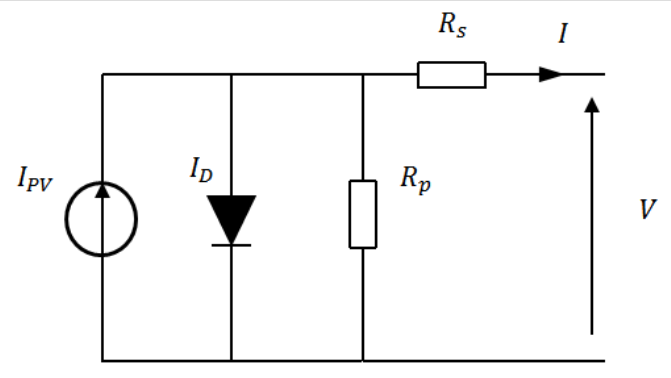
\includegraphics[width=0.9\textwidth]{./imagenes/circuito.png}
		\caption{Modelo eléctrico de los 5 parámetros}
	\end{figure}
	
	Este modelo es seleccionado ya que proporciona un buen equilibrio entre complejidad y precisión. El comportamiento matemático de este modelo se encuentra definido por la
	ecuación:
	
	\begin{equation*}
		I = I_{PV} - I_D - I_P = I_{PV} - I_0 \left ( \exp\left (  \frac{V+IR_S}{N_S \dot a \dot V_T}\right ) - 1 \right ) - \frac{V+IR_S}{R_p}
	\end{equation*}

	\section{Simulación Matlab/Simulink}
	
	Para la simulacion se divide en 4 fases:
	
	\begin{enumerate}
		\item Entradas constantes
		\item Temperatura constante e irradiancia variable
		\item Irradiancia constante y temperatura variable
		\item Entradas variables
	\end{enumerate}

	\newpage
	
	En simulink se diseño diferentes subsistemas que corresponden a cada ecuación que gobierna el modelo de la siguiente manera:
	
	\begin{itemize}
		\item Subsistema General
		
		\begin{figure}[htb]
			\centering
			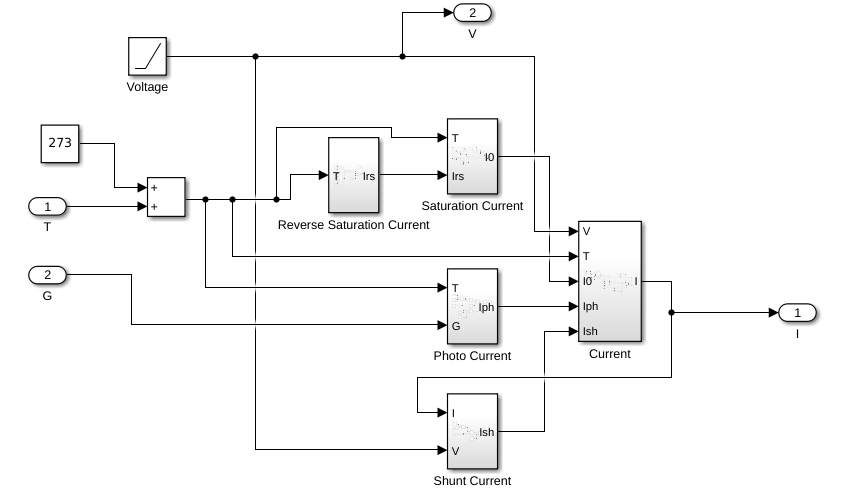
\includegraphics[width=0.9\textwidth]{./imagenes/simulink2.png}
			\caption{Sub-sistemas del modelo}
		\end{figure}
		
		
		\item Fotocorriente
		
		
		
		\begin{equation*}
			I_{ph} = \left(I_{sc} + K_i \times \left(T - 298 \right) \right) \times \left(G/1000 \right)
		\end{equation*}
		
		\begin{figure}[h!]
			\centering
			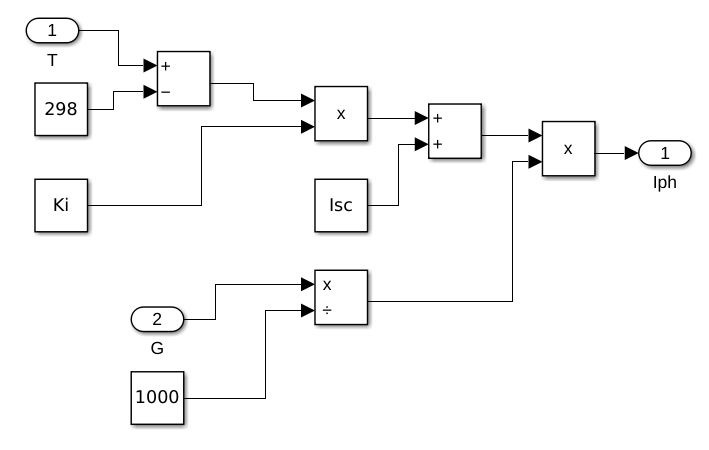
\includegraphics[width=0.55\textwidth]{./imagenes/simulink3.png}
			\caption{Subsistema para Fotocorriente}
		\end{figure} 
	
		\newpage
		
		\item Corriente de saturación
		
		\begin{equation*}
			I_o = I_{rs} \times \left( \frac{T}{T_n} \right)^3 \times \exp \left( \left( q \times E_{go} \times \left(1/T_n - 1/T \right) \right)/ \left(n \times k \right) \right)
		\end{equation*}
		
		\begin{figure}[htb]
			\centering
			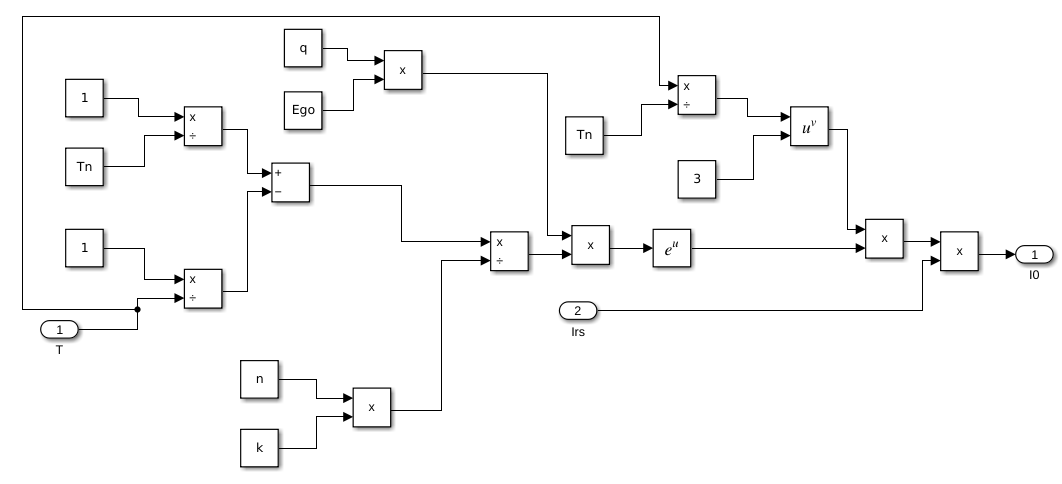
\includegraphics[width=0.9\textwidth]{./imagenes/simulink4.png}
			\caption{Subsistema de Corriente de saturación}
		\end{figure}
		
		
		
		\item Corriente de saturación reversa
		
		\begin{equation*}
			I_{rs} = I_{sc} / (\exp((q*V_{oc})/(n*N_s*k*T ))-1)
		\end{equation*}
		
		\begin{figure}[htb]
			\centering
			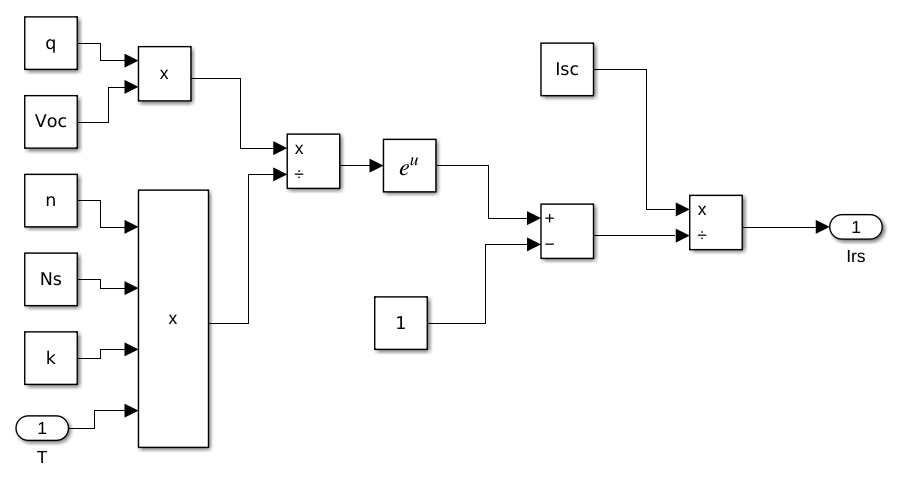
\includegraphics[width=0.9\textwidth]{./imagenes/simulink5.png}
			\caption{Subsistema de Corriente de saturación reversa}
		\end{figure}
		
		\newpage
		
		\item Corriente shunt
		
		\begin{equation*}
			I_{sh} = (V +I*R_s)/R_{sh}
		\end{equation*}
		
		\begin{figure}[htb]
			\centering
			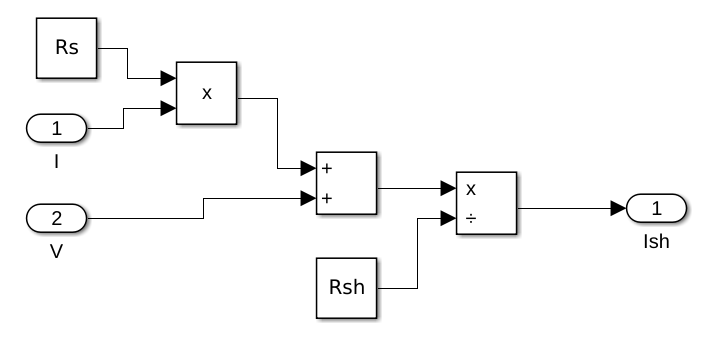
\includegraphics[width=0.9\textwidth]{./imagenes/simulink6.png}
			\caption{Subsistema de la corriente shunt}
		\end{figure} 
		
		
		\item Corriente de salida
		
		\begin{equation*}
			I = I_{ph}*NP - I_o * NP *(\exp((q*(V/NS + I*R_s/NP))/(n*N_s*k*T))-1)-I_{sh}
		\end{equation*}
		
		\begin{figure}[htb]
			\centering
			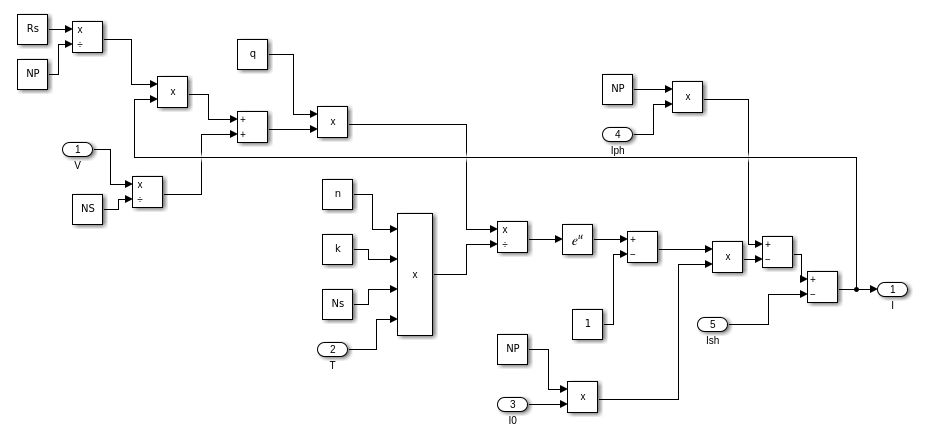
\includegraphics[width=0.9\textwidth]{./imagenes/simulink7.png}
			\caption{Subsistema de la corriente de salida}
		\end{figure} 
	\end{itemize}

	\newpage
	
	\subsection{Temperatura e Irradiancia Constante}
	
	Para esta primera simulación se considera las entradas constantes, es decir una temperatura de $25^{\circ}$C y una irradiancia de 1000 W/$m^2$
	
	\begin{figure}[htb]
		\centering
		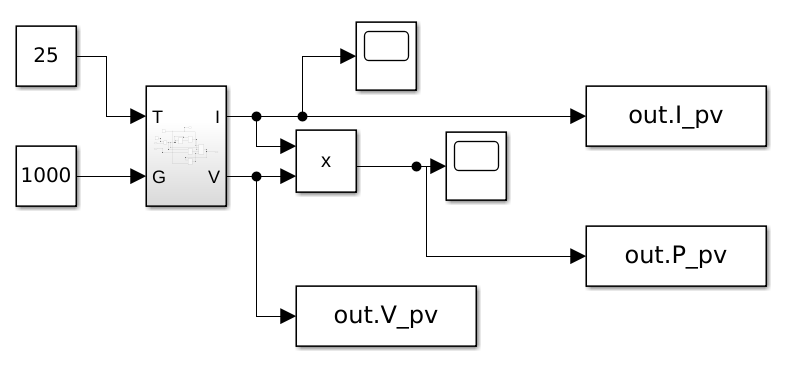
\includegraphics[width=0.9\textwidth]{./imagenes/simulink1.png}
		\caption{Arreglo PV}
	\end{figure} 
	
	Se exportan los resultados generados y se guardan de manera local en un archivo: \textit{outputPV.txt}, el cual consta de dos columnas de datos recolectados de la tension y la corriente del arreglo fotovoltaico. \newline
	
	Las curvas características que se obtienen del arreglo fotovoltaico son:
		
	\lstinputlisting[language=Python, firstline=47, lastline=82]{main.py}
		
		\begin{figure}[htb]
			\centering
			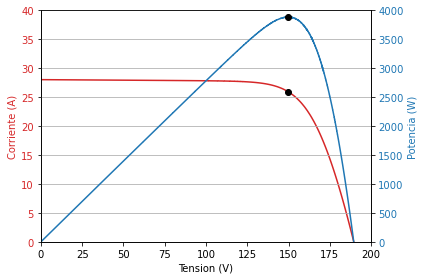
\includegraphics[width=0.8\textwidth]{./imagenes/curvacaracteristica.png}
			\caption{Curvas características}
		\end{figure} 
	
	Se extrae el punto de máxima potencia ubicado en la posición usando la siguiente función:
	
	\lstinputlisting[language=Python, firstline=34, lastline=39]{main.py}
	
	\begin{tabular}{| c | c | c | c |}
		\hline
		Indice & $V_{pv}$ & $I_{pv}$ & $P_{pv}$ \\ \hline
		149755 & 149.76 & 25.944 & 3885.37344 \\ \hline
	\end{tabular}

	\newpage
	
	Queremos obtener una función de la potencia que dependa de la tensión, $p=f(v)$ que se ajuste lo mejor posible a los valores experimentales. Una vez establecido la función a ajustar se determinan sus parámetros, en el caso de un polinomio, serán los coeficientes del polinomio de modo que los datos experimentales se desvíen lo menos posible de la fórmula empírica. \newline
	
	En python se hace uso de la función \texttt{numpy.poly1d()} que nos ayuda a definir una función polinomial de la siguiente manera:

	\lstinputlisting[language=Python, firstline=116, lastline=119]{main.py}
	
	Ahora el criterio a evaluar experimentalmente es el siguiente: 
	
	\begin{itemize}
		\item Se toma como criterio el punto de máxima potencia ubicado en el indice 149755
		\item Se crea un arreglo $\left [ 10, 20, 30, 40, 50 \right ]$ en donde cada elemento corresponde a un rango, es decir: para el elemento $10$ entonces el rango a evaluar seria $149755 \pm  10*1000$
		\item Se crea un arreglo que corresponde a los grados de ajuste del modelo: $\left [ 3,5,7 \right ]$. Se toman grados impares ya que la curva a modelar se ajusta perfectamente a este tipo de funciones.
		\item Por lo tanto se obtiene 15 modelos polinómicos para el primer trozo de la función y otros 15 modelos para el segundo trozo.
		\item Para seleccionar la función que mejor se ajusta al modelo, se evaluá la tensión en el punto de máxima potencia y se calcula un error de aproximación para poder escoger el menor de ellos.
	\end{itemize}

	
	El resultado de los modelos para el primer trozo de la función es:
	
	\lstinputlisting[language=Python, firstline=121, lastline=193]{main.py}
	
	El resultado de los modelos para el segundo trozo de la función es:
	
	\lstinputlisting[language=Python, firstline=195, lastline=268]{main.py}
	
	Posteriormente se calcula el error de ajuste, evaluando la tensión en el punto de máxima potencia en la función obtenida, con respecto al verdadero valor de potencia máxima. Para lo cual se obtiene que los mejores modelos corresponden al modelo 10 y el modelo 0 para el primer y segundo trozo respectivamente. Por lo tanto la función final es:
	
	\begin{equation*}
		p\left ( v \right ) = \begin{cases}
			-1.481 \times 10^{-11} v^7 + 6.51\times 10^{-9}v^6 - 1.139\times 10^{-16}v^5 & \\
			+ 0.0001002v^4 - 0.004614v^3  + 0.1031v^2 + 27.05v + 2.176 & \text{ Si } 0 \leq v \leq v_{mpp} \\ 
			-0.005694v^3 - 0.04569v^2 + 412.8v - 3.7821 \times 10^{4} & \text{ Si } v_{mpp} < v \leq 200 
		\end{cases}
	\end{equation*}
	
	Si graficamos la función obtenida y la sobreponemos sobre la original (rojo) se tiene:
	
	\begin{figure}[htb]
		\centering
		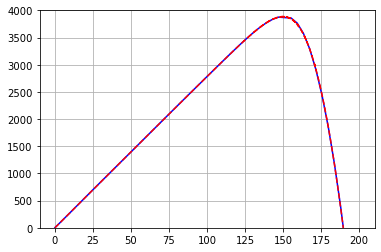
\includegraphics[width=0.8\textwidth]{./imagenes/modelo1.png}
		\caption{modelo 1 vs original}
	\end{figure}
\end{document}